\documentclass[a4paper,10pt]{article}

\usepackage[latin1]{inputenc}
\usepackage{amsfonts}
\usepackage{amsmath}
\usepackage{amssymb}
\usepackage{amsthm}
\usepackage{fontenc}
\usepackage{graphicx}
\usepackage[english]{babel}

\usepackage{listings}
\usepackage{color}
\definecolor{lightgray}{rgb}{.9,.9,.9}
\definecolor{darkgray}{rgb}{.4,.4,.4}
\definecolor{purple}{rgb}{0.65, 0.12, 0.82}

\lstdefinelanguage{JavaScript}{
	keywords={typeof, new, true, false, catch, function, return, null, catch, switch, var, if, in, while, do, else, case, break},
	keywordstyle=\color{blue}\bfseries,
	ndkeywords={class, export, boolean, throw, implements, import, this},
	ndkeywordstyle=\color{darkgray}\bfseries,
	identifierstyle=\color{black},
	sensitive=false,
	comment=[l]{//},
	morecomment=[s]{/*}{*/},
	commentstyle=\color{purple}\ttfamily,
	stringstyle=\color{red}\ttfamily,
	morestring=[b]',
	morestring=[b]"
}
\lstset{
	language=JavaScript,
	backgroundcolor=\color{lightgray},
	extendedchars=true,
	basicstyle=\footnotesize\ttfamily,
	showstringspaces=false,
	showspaces=false,
	numbers=left,
	numberstyle=\footnotesize,
	numbersep=9pt,
	tabsize=2,
	breaklines=true,
	showtabs=false,
	captionpos=b
}

\newcommand{\comment}[1]{}

\begin{document}
 \title{Documentation}
 \author{Beerend Lauwers \and Hidde Verstoep \and Frank Wijmans}
 \maketitle

 \section{Introduction}
 We have used the HJS Javascript library as found on Hackage. 
 We noticed that not all datatypes defined in the library were actually used as a (partial) result in the parsing process. 
 We translated the generated AST to our own AG AST (defined in \texttt{Datatypes.ag}) in \texttt{Convert.hs}. 
 As a result, our AG does not contain all the datatypes from the library.
 
 We have analysed Javascript code using Attribute Grammars in Haskell.
 The purpose of our analysis is to find out about the possible typing of variables and functions, since Javascript is a dynamic and weakly typed language.
 This document provides information about the following source code files:
 \begin{enumerate}
 	\item \texttt{Attributes.ag} 
 	
 	Basic attributes are defined here.
 	\item \texttt{Datatypes.ag} 
 	
 	Contains our AG datatypes based upon those of the parser.
 	\item \texttt{Flow.ag} 
 	
 	The edges and vertices of the flow graph are built here.
 	\item \texttt{Scope.ag} 
 	
 	Special attention for scoping, i.e. attending to the details of variables and functions.
 	\item \texttt{Transfer.ag} 
 	
 	Transfer functions are defined here for use in the analysis algorithm. The algorithm is named \texttt{alg} in the source code.
 	\item \texttt{Convert.hs} 
 	
 	The conversion between parser and the 'ag-datatypes'.
 \end{enumerate}

 To use our analysis on a Javascript file, first you have to build the executable using the \texttt{make} command.
 Then, use the following command to generate a *.png/*.pdf file: \texttt{test.sh /folder/filename.js}. 
 This will generate a PDF and a PNG file of the flow graph. For example, \texttt{test.sh /examples/ltgt.js} will generate the files \texttt{ltgt.dot.png} and \texttt{ltgt.dot.pdf}.
 
 \section{Flow Graph}
 We generate an image of a directed flow graph, starting at \texttt{program-begin} and ending at \texttt{program-end}. 
 Black edges simply follow evaluation order (as defined in \cite{ecma}).
 Red edges denote interprocedural edges. Green edges point from a call program point to the return program point and are only included to improve readability.
 
 \section{Transfer functions}
 Transfer functions are generated for all edges of the flow graph, after which they are added to the work list.
 The work list algorithm then calculates all the types a certain program point may have. 
 The algorithm and transfer function code is defined in \texttt{Transfer.ag}.

 \section{Lattice}
 Our lattice code can be found in \texttt{Transfer.ag}. We have chosen a lightweight implementation using a \texttt{Lattice} Haskell type class, of which instances were made for sets, where our \texttt{join} operator is set union and our \texttt{meet} operator is set intersection, and one for the Data.Map datatype, where \texttt{join} and \texttt{meet} are respectively \texttt{Data.Map.unionWith join} and \texttt{Data.Map.intersectionWith meet}; the \texttt{join} and \texttt{meet} functions are those of the values of the Map.
 We define a simple datatype type \texttt{Type} that contains the types we are able to infer.
 Our lattice is then defined as a set of primitive types: \texttt{type TLattice = Set Type}.
 We then define a type synonym for use in our transfer functions: \texttt{type Data = Map Vertex TLattice}.
 Our transfer functions go from \texttt{Data $ \rightarrow $ Data}.

  \section{Examples}
 \subsection{Poisoning.js}
 Unfortunately our analysis is not context-sensitive. 
 The code in figure \ref{poisoningCode} is subject to poisoning, as can be seen in the generated graph in figure \ref{poisoningGraph}.
 The infered types of \texttt{x} and \texttt{y} are the same.
  
 \begin{figure}[h!]
 \lstinputlisting{../examples/poisoning.js} 
 \caption{Javascript code - poisoning.js}
 \label{poisoningCode}
 \end{figure}
 
 \begin{figure}
 	\begin{center}
 	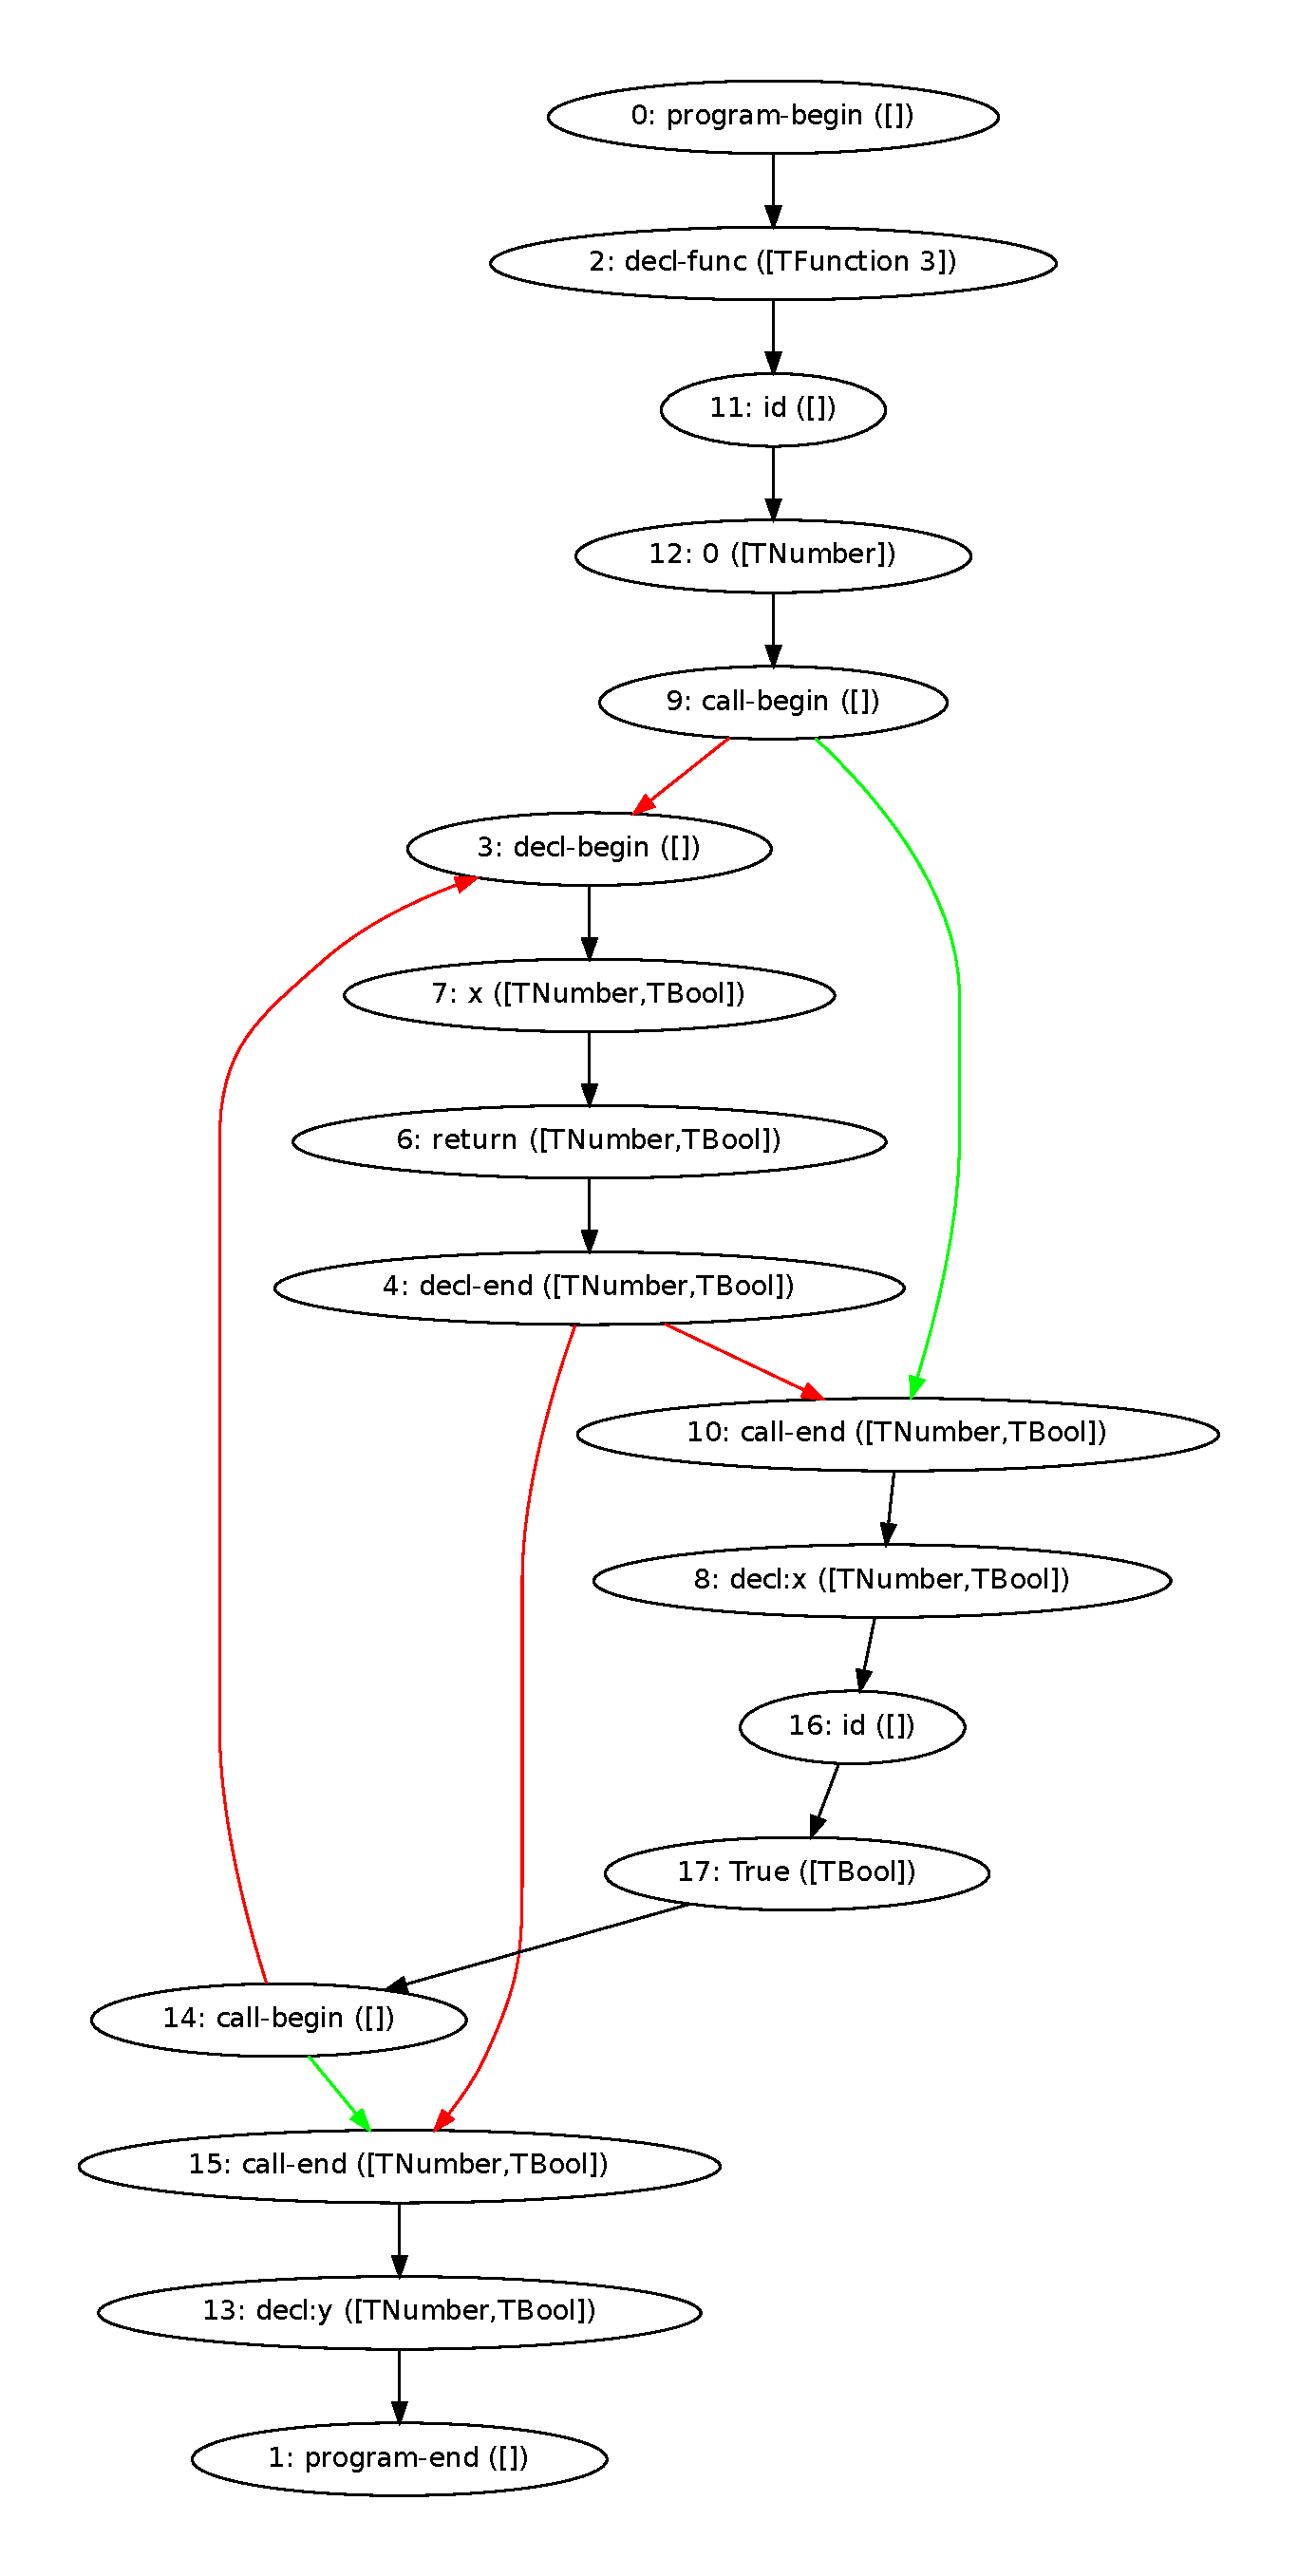
\includegraphics[height=\textheight]{../examples/poisoning.pdf}
 	\caption{The graph image generated from poisoning.js}
 	\label{poisoningGraph}
	\end{center}
 \end{figure}

 
 \subsection{Ltgt.js}
 The Javascript code in figure \ref{ltgtCode} has two functions and a while loop using these two functions.
 Notice the difference in defining the functions and the usage of the variable y.
 
 \begin{figure}
 \lstinputlisting{../examples/ltgt.js} 
 \caption{Javascript code - Ltgt.js}
 \label{ltgtCode}
 \end{figure}
 
 To show how this is formulated in the analysis, let's walk through the generated graph and draw the links between code and result.
 
 \begin{figure}
 	\begin{center}
 	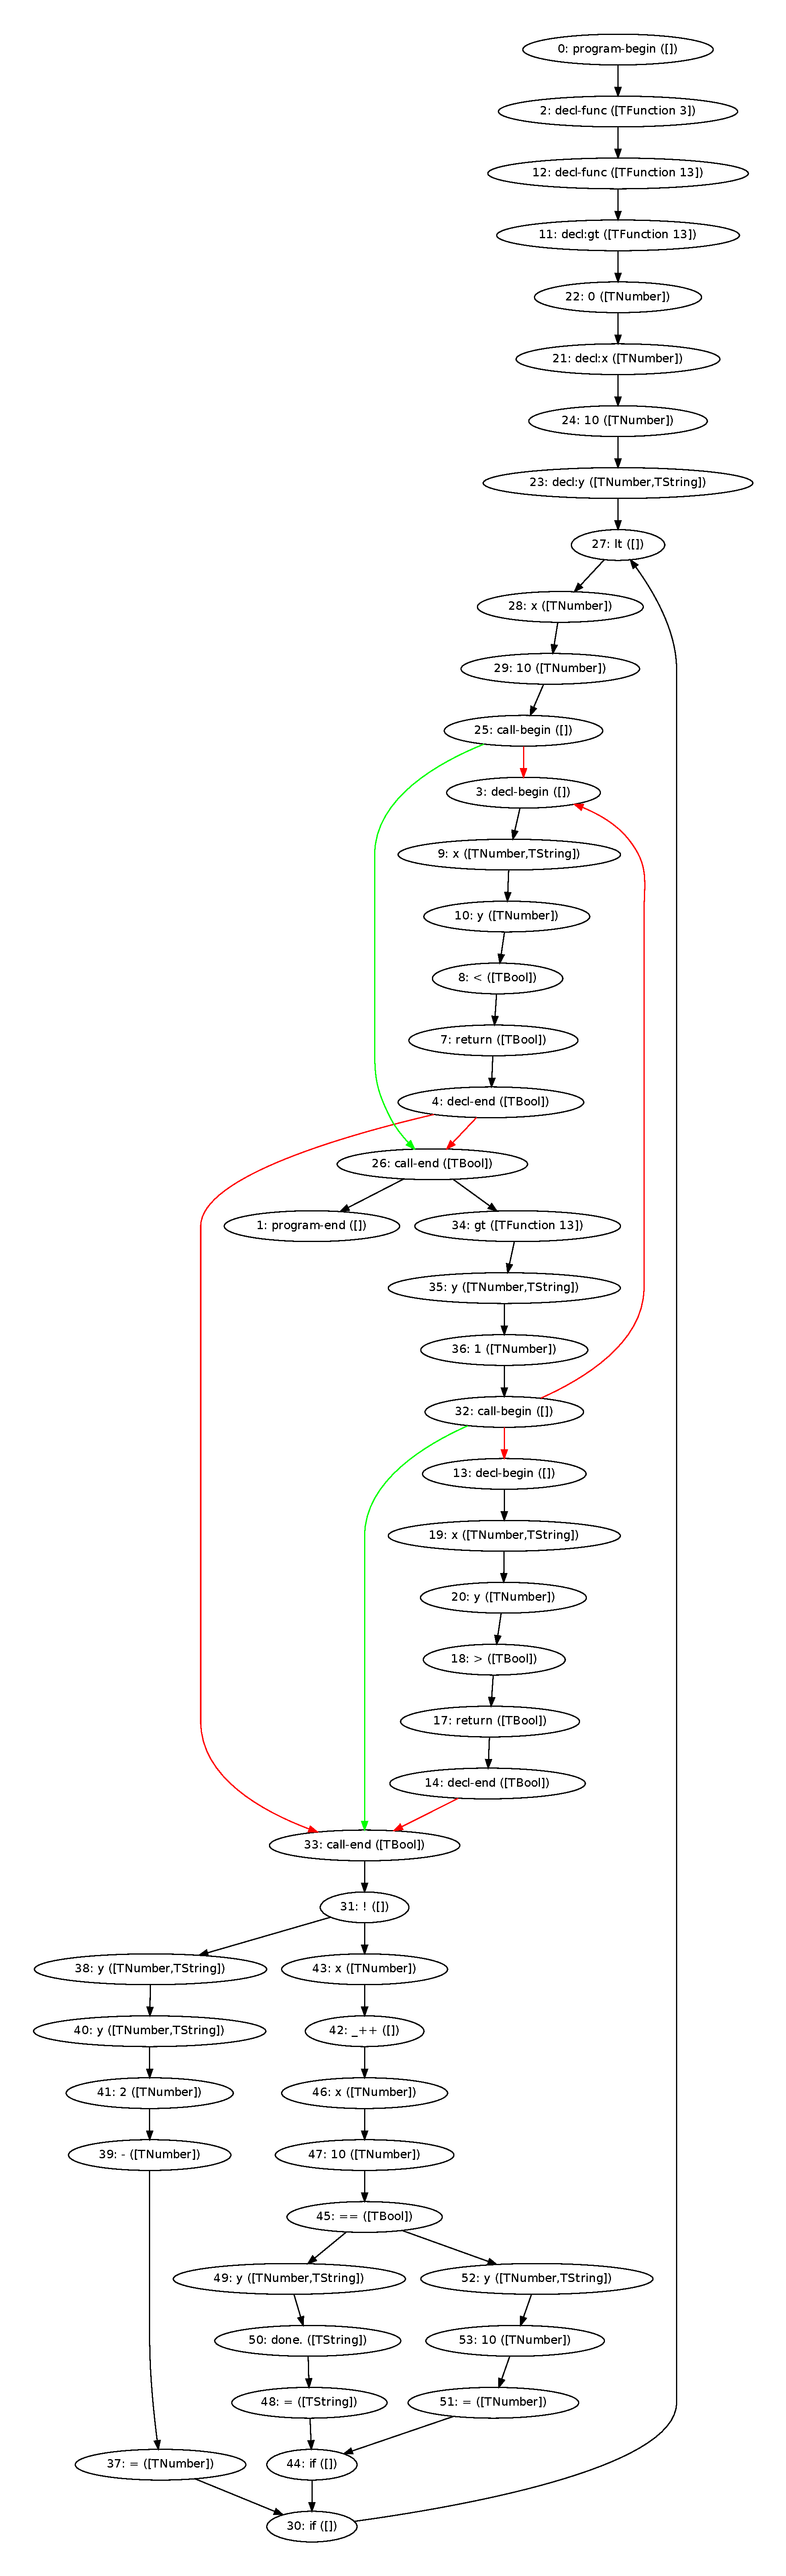
\includegraphics[height=\textheight]{../examples/ltgt.pdf}
 	\caption{The graph image generated from Ltgt.js}
 	\label{ltgtGraph}
	\end{center}
 \end{figure}

 The function of the code snippet might be a little trivial, but a few language concepts are encapsulated within this example.
 \begin{enumerate}
 	
 	\item Variables that contain more than one type. 
 	In this example it is clear that the two following assignments will not infer the same type.
 	\begin{lstlisting}
 		var y = 10;  \\ TNumber
 		y = "done."; \\ TString
 	\end{lstlisting}
 	
 	\item Variable names are shadowed.
 	We use \texttt{x} and \texttt{y} in the global scope, but we also shadow these inside the functions \texttt{gt} and \texttt{lt}. 
 	We even mix up \texttt{x} and \texttt{y} to show the scoping rules are correct.
 	
 	\item Function declaration styles.
 	\begin{lstlisting}
         function lt (x,y) {...}   \\ TFunction
var gt = function    (x,y) {...};  \\ TFunction
 	\end{lstlisting}
 	First up is the usual way of declaring functions, where the top level gets access to the function (in other words, it becomes globally accessible).
 	Secondly we have an anonymous function declaration that we assign to a variable.
 	There is a subtle difference in the flowgraph. 
 	When \texttt{lt} is called we can add an edge to the function declaration. 
 	When \texttt{gt} is called however, we have to add edges to all function declarations because we do not know to which function a variable might refer.
 		
 \end{enumerate}

 When looking at the graph we see that it closely follows the code.
 From nodes 0 to 23 we find the declaration of two functions and the assignment of \texttt{gt}, as well as the initialization of \texttt{x} and \texttt{y}, and respectively their first assignments.
 
 The call of \texttt{lt} is on node 25 on the values \texttt{x} and \texttt{10}.
 Continuing into the loop body, something interesting happens: 
 on node 9 you see the first shadowing due to scoping, namely on the name \texttt{x}.
 Let us use \texttt{x'} to denote that it is a shadowed \texttt{x}.
 Node 23 states that \texttt{y} is a number and a string during the entire run of the program.
 As this top-level \texttt{y} is passed to the \texttt{gt} function in the first \texttt{if} construct, the types of \texttt{x'} become the same as those of \texttt{y}.
 
 Having called \texttt{gt}, we take the negation of the resulting value. This is visible in node 31.
 Following the structure, the interesting part happens in the \texttt{if} construct inside the outer \texttt{else} branch. We see here that \texttt{y} is assigned either ``done.''(node 48) or 10 (node 51).
 Node 44 shows the end of the inner \texttt{if} construct, and node 30 does the same for the outer \texttt{if} construct, after which program flow goes back to node 27 to begin another iteration of the \texttt{while} loop.
 
 \section{Future Work}
 Our analysis cannot accurately analyse objects and higher-order functions. 
 To construct a more precise flowgraph for higher order functions, another analysis could be performed.
 Another analysis would be to do partial evaluation, so we could analyse objects.
 It would also be interesting make our analysis context-sensitive to avoid poisoning.
 
 \bibliographystyle{ieeetr}
 \bibliography{Documentation}
 
 
\end{document}
